\documentclass[preprint,12pt]{elsarticle}
\linespread{1}
\usepackage{amssymb}
\usepackage{lineno}
\usepackage[margin=0.5 in]{geometry}
\usepackage[utf8]{inputenc}
\usepackage{amsmath}
\usepackage{graphicx}
\usepackage{epstopdf}
\usepackage{lmodern}
\usepackage{caption}
\graphicspath{ {figures/} }

\newcommand{\exedout}{%
  \rule{0.8\textwidth}{0.5\textwidth}%
}
\begin{document}

\begin{frontmatter}

\title{FlexPass: Incentive Prompts for Reducing on-campus Parking Demand}

\author{Dounan Tang, Ziheng Lin,}

\address{University of California, Berkeley}

\begin{abstract}
%% Text of abstract

\end{abstract}


\begin{keyword}
Parking \sep Incentives \sep Randomized Controlled Trial \sep Casual Inference \sep 
%% keywords here, in the form: keyword \sep keyword

%% MSC codes here, in the form: \MSC code \sep code
%% or \MSC[2008] code \sep code (2000 is the default)
\end{keyword}

\end{frontmatter}

\section{Introduction} (7-25)
In order to reduce on-campus parking demand and create a more sustainable environment, a new parking pricing strategy is being proposed by the Parking and Transportation office of University of California, Berkeley. This parking pricing strategy, named FlexPass, is to be priced to provide an incentive to park less on working days, and preferably less than four working days per week during the hours 7 am to 6 pm. Before formally launching the FlexPass into the market, an experiment was conducted during 2015-Spring semester, Feb-1-2015 to Apr-30-2015, to test the treatment effect of this new strategy. Participants in the FlexPass study will be able to claim the rebate using a smartphone app. The rebates will accumulate over the semester and be added to their July 2015 paycheck. 

\section{Description of the FlexPass Study} 
The current parking pricing system at the University of California, Berkeley (UC Berkeley) is dominated by annual or monthly parking permits. Employees purchase an annual or monthly parking permit for a lump sum cost, then they will have the incentive to drive to campus every day, since the cost of parking is not affected by their days of parking on campus. The FlexPass study is being proposed to potentially reduce the demand of parking, which could also reduce the congestion and greenhouse gas emissions from cruising for parking, as well as to encourage mode choices other than driving alone. The study runs for 2015 Spring semester, 3 months beginning on February 1, 2015 and ending on April 30, 2015.

\subsection{Experimental Design}
Currently, there are more than 20 types of campus parking permits in UC Berkeley, this project will only target the current annual Central \textbf{C} Campus Permit and Faculty/Staff \textbf{F} Permit holders who constitute the vast majority of the regular users of campus parking. These parking permits allow holders to seek a parking space in parking garages or surface lots by the permit type. 'C' permits are available only to faculty and senior staff, \textbf{F} permits to other staff. To park on campus, permit holders are required to hang their permits on the rear-view mirror. Parking enforcement is conducted by UC Berkeley Parking and Transportation officers by checking these hang tags. The current price for \textbf{F} permit is \$95 per month while \$ 131 per month for \textbf{C} permit. Participants are only allowed to take part in this study if they have already purchased a \textbf{C} or \textbf{F} permit for the entire 2015 Spring semester. Enrolled participants will be assigned into two groups, rebate and control group, through a randomized controlled trial. If assigned to the control group, participants will only be required to install the FlexPass App and report parking behavior for the entire study period. They will keep their current permit. If assigned to the treatment group, they will be asked to turn in their current hang-tag and receive an alternate one, FlexPass permit, for the study period.  \\

Participants are able to report their daily parking choices on the FlexPass App, which is available for both Iphone and Android users. App interface is shown in figure \ref{fig:app_screens}. The default setting for every day will be “Parked on Campus”. Participants can change to not park on campus for today or tomorrow on the main interface, or for several days in the future through the calendar. If participants indicate that they will not park, they will also be asked to report what alternate mode would be taking or whether they would not be coming to campus. Participants can change their parking choices for a certain day in the study period, multiple times but only till 12 noon on that day. Participants' responses regarding whether or not parking on a certain day are uploaded to the server through the FlexPass App and then sent to parking enforcement officers. If assigned to treatment group, participants may be cited if park on campus after declaring that he will not. 

\begin{figure}[!htb]
\centering
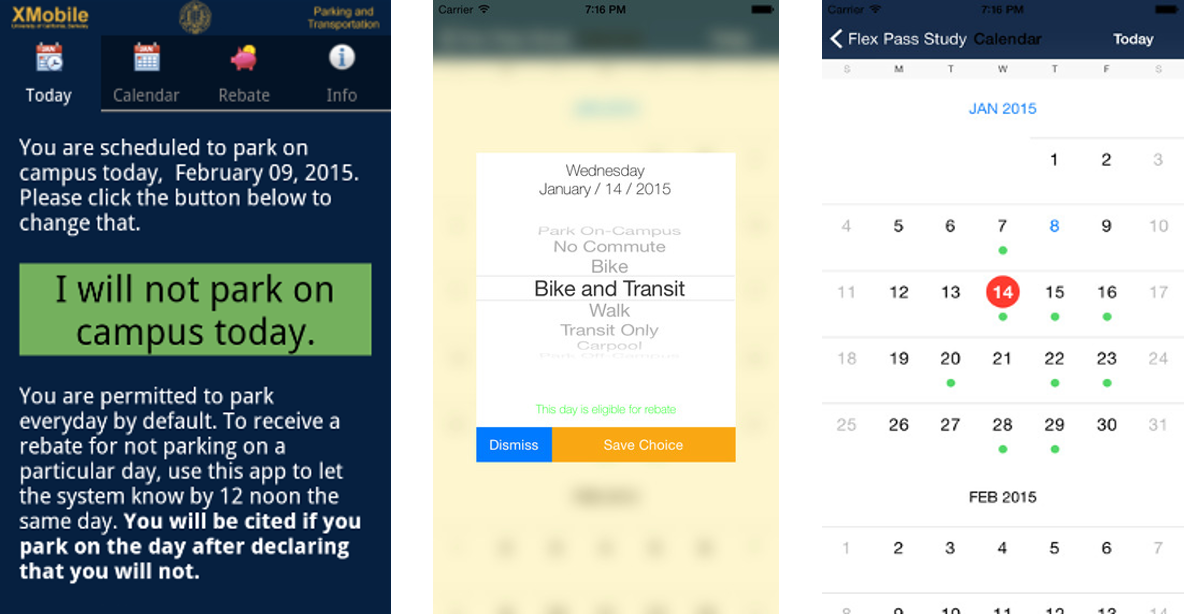
\includegraphics[scale=0.8]{app_screens.png}
\caption{FlexPass smartphone App interface. From left to right, (a) Main Screen, (b)Mode Reporting, (c) Calendar}
\label{fig:app_screens}
\end{figure}

There will be a guaranteed \$50 Amazon gift card just for participating and running the FlexPass App for the entire study period. Both group will report their daily commute modes while only rebate group is eligible for rebates which are based on their permit type and the number of working days (Mon to. Fri.) they park on campus in a given month. Rebate amounts are calculated as equation 1 below.

\[T = \max \{ \Theta  - D\delta ,0\} \]

where $D$ is the number of working days a certain participant parks on campus in a certain month and $T$ is the total rebates for that month. For that participant, the maximal rebate he or she can earn in that month is $\$\Theta$ ($\Theta$=95 for F permit holder while 131 for C permit). Every day that participant parks on campus, he or she will be changed a $\$\delta$ per day credit ($\delta$ =6 for F permit holder while 8 for C permit) until all credit has been used up. For example, as an F permit holder, if you park 12 workdays (approximately 3 work days a week), you will receive a rebate of \$23, if you park 13 days, you will receive a rebate of \$17 (i.e. \$23-\$6).\footnote{Detail description of the rebate calculation and a table of all possible rebate values can be found in the homepage of our study website https://gogreen.berkeley.edu/flexpass/.} Since participants will have already prepaid for their permit parking, the entire credit for three months will be refunded to them as a lump sum at the end of the study. 


\subsection{Sample Characteristics}

Our interested population consists of 4272 C\&F permit holders, and the enrollment was conducted through recruitment emails and postcards. 392 participants finished the sign-up procedure, where they responded to a few demographic, mobile technology and commute related questions. Then they were assigned into two groups through a randomized controlled trial, both group has sample size of 196. 

\section{Causal Analysis of the FlexPass Study}
To infer the treatment effect of the FlexPass, we proposed a box model as shown in figure \ref{fig:box_model}(a). For a certain participants indexed by $i$, his or her social economic characteristics, denoting as $X_i$ on his or her ticket, are observed through the entry survey. The ticket in the box also contains the treatment respond vector $Y_i^T$ and control respond vector $Y_i^C$. $Y_i^T$ and $Y_i^C$ is both constructed by 64 binary variables, denoting as $Y_{ij}^t$ and $Y_{ij}^c$, representing daily parking choices,which equals 1 if participant $i$ did not park on campus on day $j$ and 0 otherwise. 392 samples were drawn from the box of 4272 C\&F permit holders and assigned into treatment group and control group randomly. Let $T_i$ represents group assignment which equals 1 if assigned into treatment group and 0 otherwise. If $T_i=1$, $Y_i^T$ would be potentially observable while we observe $Y_i^C$ when $T_i=0$. We denote the overall parking choices that are supposed to be observed during the study as $\mathbf{Y}$, which is a $392\times 64$ 0-1 matrix. Under the week null hypothesis $H_0$, there is no treatment effect in the population level, which assumes the FlexPass has no effect on reducing on-campus parking demand. The purpose of our causal analysis is evaluate the size and variance of the treatment effect $\overline {\sum\limits_j \mathbf{{{Y^t}_{ij}}} }  - \overline {\sum\limits_j \mathbf{{{Y^c}_{ij}}} } $ to decide whether we can reject the null hypothesis at certain confidence level. However, problem arisen during the study as not all $Y_{ij}$s are observed, which causes biases in causal analysis. \\

In this section, missing data and dropout problems will be addressed. The missing data will be imputed by a Mixed Latent Factor Model (MLFM) while dropout bias will be compensated through selection model. The result of casual analysis will then be discussed.    

\begin{figure}[!htb]
\centering
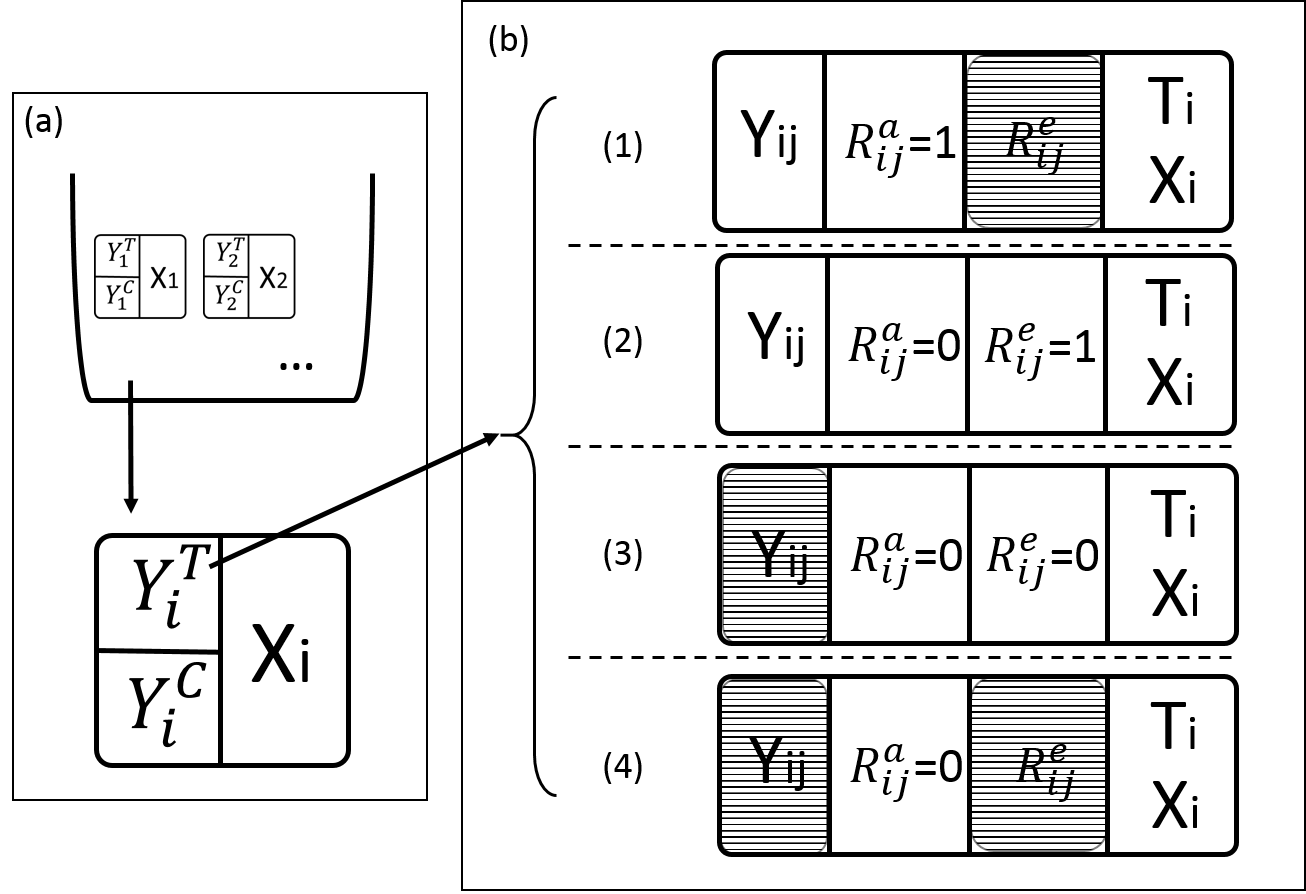
\includegraphics[scale=0.4]{box_model.png}
\caption{Box model for causal analysis}
\label{fig:box_model}
\end{figure}

\subsection{Dropouts, Missing Report Mechanism and Data Descriptions}

In order to conduct the enforcement, participants assigned to the rebate group were required to pick up their new FlexPass hang-tap at Parking and Transportation office. Only 149 participants exchanged their hang-tap and the rest 47 within the rebate group dropped out during this process. There were two participants dropped out after picked up the FlexPass because of switching to carpool and being pregnant, which further reduced the size of rebate group to 147. The App-reported longitudinal data of daily parking demand reduction of the rest 347 valid participants is shown in figure \ref{fig:Raw_time_series}. The solid lines show that on every working day, how many participants reported not parked on campus through the FlexPass App. Weekday patterns can be observed from the solid lines, e.g. during Friday the reduction of parking demand from two groups are both high. There are two outliers showing up on Monday Feb-016-2015 (President day) and Friday Mar-27-2015 (Cesar Chavez Day). They are considered as Academic and Administrative Holidays in UC Berkeley and excluded from the rebate calculation. The dash lines illustrate the weekly average that deseasonalize within-week variation. Highest mean value appears in the 8th week, the Spring Recess, when faculties have no course to teach but staffs work as usual. Note that the blue line which represents the treatment group is always above the green line which represents the control group. This may be a indicator for significant treatment effect at the first sight. However, this comparison relies on a strong assumption that when people did not report any thing through the App on certain days, they are considered as "Park On Campus". In fact, from focus group interviews during the study, we learned that there were considerable number of days participants forgot to use the App when did not use campus parking. Especially for participants in control group, since there is no incentives for them to report daily commute modes, from the beginning (Feb-01-2015) to the end (Apr-31-2015) there are 74 participants in the control group have reported nothing through our smartphone App. Even with participants who have reported some choices, they may still under report the number of not-park-on-campus days, which leads to an overestimation of the treatment effect. Therefore, instead of respond $Y_{ij}$, we additionally define, for each occasion j, an indicate $R_{ij}^a$, which equals 1 if participant $i$ reported day $j$'s parking behavior through smartphone App and 0 if participant $i$ didn't use the App on day $j$. We then partition $Y_i$ into two sub-vectors such that $Y^o_i$ is the vector containing those $Y_{ij}$ for which $R_{ij}^a=1$ and $Y^m_i$ contains the remaining components. $Y^m_i$ is referred to missing reports. To further understand the missing report process, we sent commute mode surveys among 6 weeks during the study period. Our system sends survey links through follow-up emails to our participants who had not used their smartphone App for a week prior to the survey. The survey let participants choose whether they parked on campus or not on each day in the past week. The average respond rate for the email survey is 66 $\%$. Hence for each occasion j, another indicator is defined as $R_{ij}^e$, which equals 1 if participant $i$ reported day $j$'s parking behavior through email and 0 otherwise.\\

 \begin{figure}[!htb]
\centering
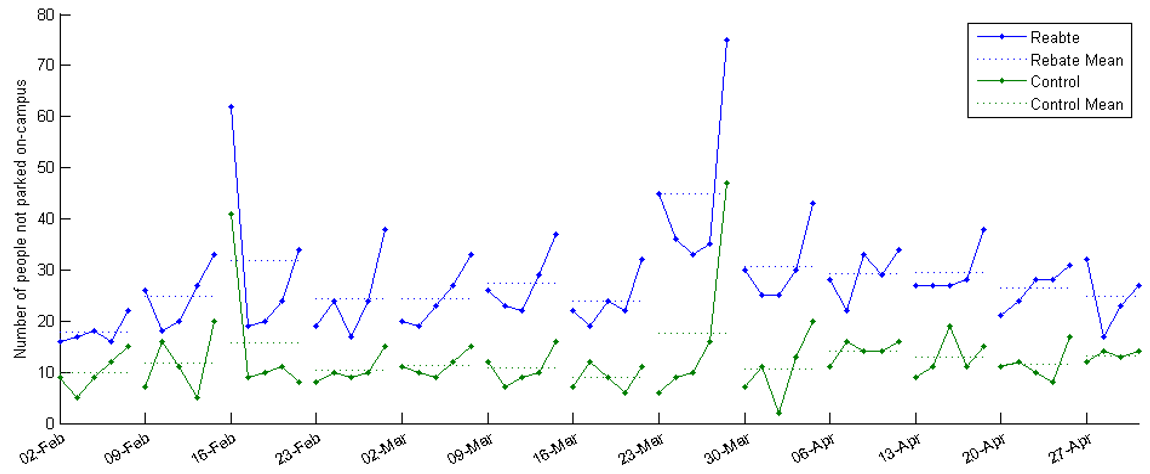
\includegraphics[scale=0.6]{AppReportRaw.png}
\caption{Daily on-campus parking demand reduction for rebate and control groups}
\label{fig:Raw_time_series}
\end{figure}

From the email survey, a hypothesis testing of the missing report mechanism was conducted among three alternates, i.e. Missing Completely At Random (MCAR), Missing At Random (MAR), and Missing Not At Random (MNAR) [Rubin 1976, Little and Rubin 1987]. The three mechanisms differ from each other based on the dependencies between missingness and observed and unobserved data. MCAR refers to the missingness is independent of both observed and unobserved data; MAR refers to missingness is independent of unobserved data; MNAR refers to missingness is independent of neither observed or unobserved data. The missingness process for MCAR and MAR are ignorable such that we can ignore formulating the missingness process when we are inferring the treatment effect. Otherwise, if the MNAR holds we should model the missingness process before conducting causal analysis. In FlexPass study, since the all participants understand that default setting on the App is "Park on Campus", a possible evidence of MNAR could be people parked more on campus tend to use the App less often and are missing on App reports. Hence MAR and MNAR can be distinguished by comparing the parking behavior reported from follow-up emails with App reports. The bar chart figure \ref{fig:AverageParkingBarPlot} illustrates average number of days participants did not use campus parking in those 6 weeks. It can be observed that the email responds of non-campus parking days is generally lower than the App reports. For all 6 weeks, the App reports resulted in averagely 1.92 non-campus parking days per week among the rebate groups, while this number is 0.57 for email responds. Through a two sample t-test the null hypothesis of MAR leads to a p-value of 0.002 , which rejects MAR and also MCAR. The missing report mechanism is regarded as MNAR and will be modeled through a Mixed Latent Factor Model (MLFM) in the next section.


\begin{figure}[!htb]
\centering
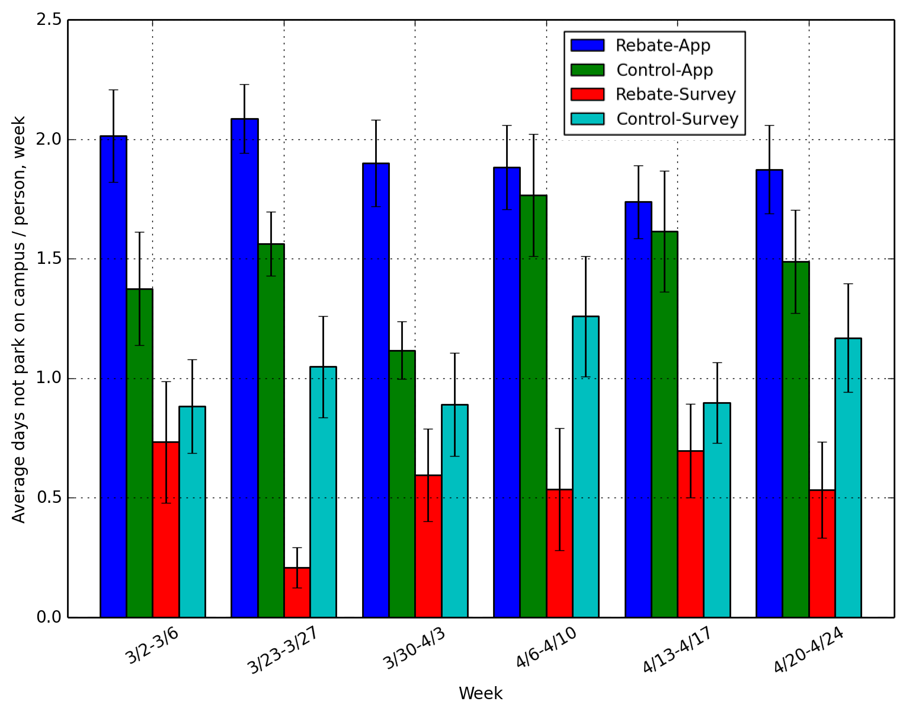
\includegraphics[scale=0.4]{AverageParkingBarPlot.png}
\caption{Comparison of non campus parking days between App reports and email responds }
\label{fig:AverageParkingBarPlot}
\end{figure}
 

To sum up, in our study, respond vector $Y_i$ is measured through both App and follow-up email system. All possible outcomes for $Y_{ij}$ are then illustrated in figure \ref{fig:box_model}(b), where the shaded region means not observable. In situation (1), participant i report day j's parking choice through the App, where $Y_{ij}$ is observed and no email will be sent. In situation(2) , participant i didn't use the App on day j and an email will be sent to i. He or she answered the email and thus $Y_{ij}$ is observed. In situation(3), $Y_{ij}$ is not observed as participant i didn't answer the email. As emails are only sent out for six weeks, situation(4) may also happen, where participants i would not receive any email even he didn't use the App for certain days. Or participants i belongs to treatment group but dropped out when asked to change hang tag. He or she will uninstall the App and never appears in the email list. Noticeably, all $Y^o_i$ is observed in this study by definition and part of $Y^m_i$ is measured in situation (2). If $Y_i$ only contains $Y_{ij}$ of situation (3) and (4), participants i is regarded as 'Dropout Participants'. Otherwise, complete data $Y_i$ will be recovered from $Y_{ij}$ observed in situation (1) and (2).\\

\subsection{Recover Missing Reports} 
In transportation studies, feature based models especially linear regressions is often used for interpretation and prediction. Feature based models utilize participants' demographic information and characteristics of alternatives to predict participants' choices under certain situation. In the most simple case, $Y_{ij}$ can be fitted by a linear model as
\begin{equation}\label{eq:Y_UV}
{Y_{ij}} = {\mathbf{U_i}}'{\mathbf{V_j}} + {\varepsilon _{ij}}
\end{equation}

where $\mathbf{U_i}$ and $\mathbf{V_j}$ are L dimension vectors. In models based on concrete attributes, $\mathbf{U_i}$ may be L distinct characteristics for participants $i$, e.x. age, income and gender, while $\mathbf{V_j}$ may be corresponding coefficient vectors of day $j$, e.x. $\mathbf{V_j}$ may be different for Fridays and Mondays. However, the demographic information that was acquired from study participants is limited and lack of granularity so it is not able to capture all heterogeneities of participants' behavior. In the FlexPass study, we surveyed the participants for their demographic information (age, gender, income, and etc.) and commute habits (day of driving, transit, and etc.) in the entry survey introduced in section 2. The survey resulted 21 attributes that can be included in attribute based model. Even with such many attributes, 26 participants had entirely duplicated attributes to one or more others. The commute behavior of those 26 participants turned out quite differently, which is difficult to be measured by feature based models. For attributes of weekdays, we could utilize average temperature and precipitation. However, the rather stable weather in the bay area would not help differentiating different commute choices. Personal schedules and preferences along with special events on campus, which is not observed in the study, would affect largely on commute mode choices. Moreover, if instead of interpretive ability we care more about predicting accuracy, there will be better candidates of $\mathbf{U_i}$ than social economic features, which give rise to Latent Factor Model(LFM).\\     

The Latent Factor Model(LFM) is widely applied in recommendation systems in the movie and music industry for matching users and potential items that they would be interested in. The users' rating towards items will be stored in a rating matrix which is often very sparse. The idea behind LFM is that preference of a user and attitudes of a item are determined by a small number of unobserved factors. These latent factors are capable utilizing observed user-item interactions for predicting unobserved interactions with good performances. \\

Applying the concept to the FlexPass study, we regard the study participants and the working days during the study period as 'users' and 'items', while parking choice matrix $Y$ as rating matrix. Denote the number of participants as M and number of working days as N. $Y_{i,j}$ stores participant i's parking choice on day j. 
To illustrate the idea of LFM, we first assume for all i and j, $Y_{ij}$ is generated by from the same process described in equation \ref{eq:Y_UV} with  $\mathbf{U}$ and $\mathbf{V}$ unknown. $\mathbf{U}$ and $\mathbf{V}$ is a $M\times L$ and $N\times L$ matrix respectively, where $i^{th}$ row of $\mathbf{U}$ is referred as participant i's latent factor while $j^{th}$ row of $\mathbf{V}$ is referred as day j's latent factor. When $\varepsilon _{ij}$ is independent and identically Gaussian distributed (i.i.d. Gaussian), the estimated parking respond matrix $\hat{Y}$ can be expressed by $\mathbf{U}'\mathbf{V}$. Let ${\left\| . \right\|_F}$ denotes Frobenius norm, to maximize the prediction accuracy of rating matrix equals to solve:

\[{\min _{rank(\widehat {\mathbf{Y}}) \leqslant {\text{L}}}}{\left\| {{\mathbf{Y - }}\widehat {\mathbf{Y}}} \right\|_F}\]
whose solution is essentially a singular value decomposition(SVD) of $\mathbf{Y}$. Optimal $\hat{\mathbf{Y^*}}$ and corresponding prediction error can be expressed by:
\[\hat {\mathbf{Y^*}} = \sum\limits_{i = 1}^L {{\sigma _i}{u_i}{v_i}'} ;\;\;{\left\| {{\mathbf{Y - \hat Y^*}}} \right\|_F} = \sum\limits_{i = L + 1}^{rank({\mathbf{Y}})} {{\sigma _i}^2} \]
where $\sigma_i$ is known as $i^{th}$ singular values of $\mathbf{Y}$, $u_i$ and $v_i$ is called the $i^{th}$ left-singular vector and right-singular vector, respectively. These singular vectors are often regarded as latent semantic factors in information retrieval. In the FlexPass study, the full dataset should contain 292*64=18688 responds, while in the real-world we collected 8093 App responds and 2609 email responds, which account for 57$\%$ of the full dataset size. Since the sum-square distance can be computed only for the observed entires of the target sparse matrix $\mathbf{Y}$, as shown by, this seemingly minor modification results in a difficult non-convex optimization problem which cannot be solved using standard SVD. LMF is closely related to SVD but models directly the observed ratings while avoid overfitting through a regularized model. To learn the latent vectors, the standard LFM minimizes the regularized squared error on the set of known ratings:  

\[\min_{U,V}\sum\limits_{i, j}(Y_{ij} -  U_i' V_j)^2 + \lambda (\|U \|_F + \|V \|)_F\] 

where $\lambda$ is the regularization parameter which is tuned using cross-validation. As described before, the key underlying probabilistic foundation for LFM is that the error term in equation \ref{eq:Y_UV} is i.i.d. Gaussian which implies the missing data mechanism is considered as MCAR. 
\\

To model MNAR mechanism, we proposed a Mixed Latent Factor Model(MLFM), where $Y_{ij}$ generated from two different processes depending on whether $Y_{ij}$ is observed through App reporting, ${R^a}_{ij}=1$, or otherwise ${R^a}_{ij}=0$.
 
\begin{equation}\label{eq:MLFM}
{Y_{ij}} = (1 - {R^a}_{ij}){\alpha ^m}_i + {R^a}_{ij}{\alpha ^o}_i + {\beta _j} + {{\mathbf{U}}_{\mathbf{i}}}{\mathbf{'}}{{\mathbf{V}}_{\mathbf{j}}} + {\varepsilon _{ij}};\;\;{\varepsilon _{ij}} \sim \mathcal{N}(\varepsilon |0,{\sigma ^2})
\end{equation}

where $\mathcal{N}(x|\mu,\sigma^2)$ is the probability density function (pdf) of the Gaussian distribution with mean $\mu$ and variance $\sigma^2$. $R^a_{ij}$ is the App report index defined in section 3.1. The MNAR mechanism is modeled by two participant specific bias parameters. $Y_{ij}$ depends on $\alpha ^o_i$ if App report exists while depends on $\alpha ^m_i$ if otherwise. More complicated Mixed-LMF can be created where $\mathbf{U_i}$ is also different for App reports and missing reports. However, this will add $M\times L$ more parameters to the model which largely increases the computation complexity. Also, absorbing all heterogeneities of App report responds $Y^o_i$ and missing reports $Y^m_i$ by two M dimension vectors leads to more clear interpretations. To prevent over-fitting, we also place zero-mean spherical Gaussian priors on latent factors:
\[p({\alpha ^o}|{\sigma _{{\alpha ^o}}}^2) = \prod\limits_{i = 1}^M {\mathcal{N}({\alpha ^o}_i|0,{\sigma _{{\alpha ^o}}}^2{\mathbf{I}})} ,\;\;p({\alpha ^m}|{\sigma _{{\alpha ^m}}}^2) = \prod\limits_{i = 1}^M {\mathcal{N}({\alpha ^m}_i|0,{\sigma _{{\alpha ^m}}}^2{\mathbf{I}})} ,\;\;p(\beta |{\sigma _\beta }^2) = \prod\limits_{j = 1}^N {\mathcal{N}({\beta _j}|0,{\sigma _\beta }^2{\mathbf{I}})} \]
\[p({\mathbf{U}}|{\sigma _U}^2) = \prod\limits_{i = 1}^M {\mathcal{N}({{\mathbf{U}}_{\mathbf{i}}}|0,{\sigma _U}^2{\mathbf{I}})} ,\;\;\;p(V|{\sigma _V}^2) = \prod\limits_{j = 1}^N {\mathcal{N}({V_j}|0,{\sigma _V}^2{\mathbf{I}})} \]
The corresponding graphic model for Mixed Latent Factor model is shown in figure \ref{fig:MLFM}. The log of posterior distribution over the latent factors is given by
\begin{multline*}
\ln p({{\mathbf{\alpha }}^{\mathbf{o}}}{\mathbf{,}}{{\mathbf{\alpha }}^{\mathbf{m}}}{\mathbf{,\beta ,U,V}}|{\mathbf{Y,R}},{\sigma _{{\alpha ^o}}}^2,{\sigma _{{\alpha ^m}}}^2,{\sigma _\beta }^2,{\sigma _U}^2,{\sigma _V}^2) \propto \\
\ln p({\mathbf{Y}}|{\mathbf{R}},{{\mathbf{\alpha }}^{\mathbf{o}}}{\mathbf{,}}{{\mathbf{\alpha }}^{\mathbf{m}}}{\mathbf{,\beta ,U,V}}) + \ln \prod\limits_{i,j} {\mathcal{N}{{({\alpha ^o}_i|0,{\sigma _{{\alpha ^o}}}^2{\mathbf{I}})}^{{R^a}_{ij}}}}  + \ln \prod\limits_{i,j} {\mathcal{N}{{({\alpha ^m}_i|0,{\sigma _{{\alpha ^m}}}^2{\mathbf{I}})}^{(1 - {R^a}_{ij})}}} \\
 + \ln p({\mathbf{\beta }}|{\sigma _\beta }^2) + \ln p({\mathbf{U}}|{\sigma _U}^2) + \ln p({\mathbf{V}}|{\sigma _V}^2)
\end{multline*}
Maximizing the log-posterior over latent factors with hyper-parameters, i.e. prior variances, kept fixed is equivalent to minimizing the sum-of-squared-errors objective function with quadratic regularization terms. Furthermore, to control the number of hyper-parameters,we set $\sigma_{\alpha^o}$=$\sigma_{\alpha^m}$= $\sigma_{\beta}$ and $\sigma_U$=$\sigma_V$.
\begin{multline}
\min \sum\limits_{i,j} {{I_{ij}}\{ {{[{Y_{ij}} - (1 - {R^a}_{ij}){\alpha ^m}_i + {R^a}_{ij}{\alpha ^o}_i + {\beta _j} + {{\mathbf{U}}_{\mathbf{i}}}{\mathbf{'V}}]}^2}} \\ + {\lambda _{\alpha \beta }}[{R^a}_{ij}{\alpha ^o}{_i^2} + (1 - {R^a}_{ij}){\alpha ^m}{_i^2} + {\beta _j}^2] + {\lambda _{UV}}({U_{ij}}^2 + {V_{ij}}^2)\} 
\end{multline}
where $I_{ij}$ is the indicator function of all observed data that $I_{ij}=R^a_{ij}+R^e_{ij}$ and $\lambda_{\alpha \beta}=\sigma^2/\sigma_{\beta}^2$, $\lambda_{UV}=\sigma^2/\sigma_{U}^2$. A local minimum of the objective function given by equation can be found by perform gradient descent in ${{\mathbf{\alpha }}^{\mathbf{o}}}{\mathbf{,}}{{\mathbf{\alpha }}^{\mathbf{m}}}{\mathbf{,\beta ,U}}$ and $\mathbf{V}$.\\

\begin{figure}[!htb]
\centering
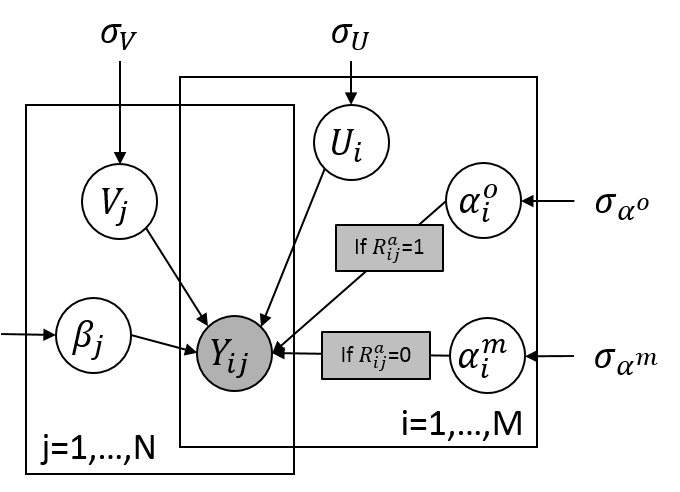
\includegraphics[scale=0.6]{MLFM.png}
\caption{Graphic Model for Mixed Latent Factor Model}
\label{fig:MLFM}
\end{figure}

`Dropout Participants' were first removed, which results in 271 valid users in our MLFM, M=271. All weekdays during the study are included, which leads to N=64. Dimension of latent factors L is set to be 10. As we penalize the norms of parameters, the model performance will not be sensitive to L.   At the occasion {i,j} where the respond is missing, we predict that participant i will not park on campus on day j if the $\mathbf{Y}$ estimated from equation \ref{eq:MLFM} is larger than 0.5. A 5-fold cross validation was conducted to choose optimal $\lambda_{UV}$ and $\lambda_{\alpha \beta}$. The original sample is randomly partitioned into 5 equal sized subsamples. Every round, a single subsample is retained as the validation data for testing the model, and the remaining 4 subsamples are used as training data. The cross-validation process is then repeated 5 times and the 5 predicting errors can then be averaged to produce a single estimation called cross validation error. $\lambda_{\alpha \beta}=0.5$  and $\lambda_{UV}=0.05$ results in the best overall cross validation error of 20.88$\%$. For participants in control group, the false positive rate $p({{\hat Y}_{ij}} = 1|{Y_{ij}} = 0,T_i=0)$ is 19.07$\%$ while the false negative rate $p({{\hat Y}_{ij}} = 0|{Y_{ij}} = 1,T_i=0)$ is 18.09$\%$. For participants in treatment group, the false positive rate $p({{\hat Y}_{ij}} = 1|{Y_{ij}} = 0,T_i=1)$ is 13.61$\%$ while the false negative rate $p({{\hat Y}_{ij}} = 0|{Y_{ij}} = 1,T_i=1)$ is 25.39$\%$. Although the false positive and negative rate is balanced for treatment population, it systematically under-predicts the number of non-campus parking days, which will lead to a conservative estimation of treatment effect. \\

In the estimated model, there are L dimensions latent components in both $\mathbf{U}$ and $\mathbf{V}$. Similar to the standard SVD, we rank these components by their information amount, where first calculate ${\sigma _l}^2 = \sum\limits_{i = 1}^M {{U_{il}}^2}  + \sum\limits_{j = 1}^N {{V_{jl}}^2}$, and sort $\mathbf{U}$ and $\mathbf{V}$ in the way that ${\sigma _l^2}\geqslant {\sigma _{l+1}^2}$ for all $l=1,...,L$. $l^{th}$ column of the new $\mathbf{V}$ is denoted as $l^{th}$ principal component of $\mathbf{V}$. Weekday latent factor matrix $\mathbf{V}$ is visualized by its first and second principal component in figure \ref{fig:VFirstTwo}. Different weekdays are drawn with different color and markers. Patterns can be observed such as Fridays are mainly distributed on the upper part while Mondays on the lower left. Features of two holidays are captured in the model as their latent factors departs from the population. In order to show how MNAR mechanism is captured in participant specific bias parameters, ca scatter-hist plot for $\alpha^o_i$ and $\alpha^m_i$ is drawn for every valid participant i on figure \ref{fig:AlphaMO} showing The kernel density for both $\alpha^o$ and $\alpha^m$ is also illustrated near x and y axis respectively. It can be observed form the scatter plot that for participants in treatment group, most of the blue dots are below the 45 degree dash line, meaning that $\alpha^o_i>\alpha^m_i$, which is in line to with the information shown in figure \ref{fig:AverageParkingBarPlot}. From the kernel density plot for $\alpha^o$ we can observe that the distribution of $\alpha^o$ for treatment group is shifted to the right of control group, meaning the App reposts revealed that treatment group forgone parking on campus more often. However, focusing on the kernel density plot for $\alpha^m$, $\alpha^m_i$ for treatment group are concentrating at rather low values, while $\alpha^m$ distribution of control group shows similar pattern as its  $\alpha^o$ distribution. 

\begin{figure}[!htb]
\centering
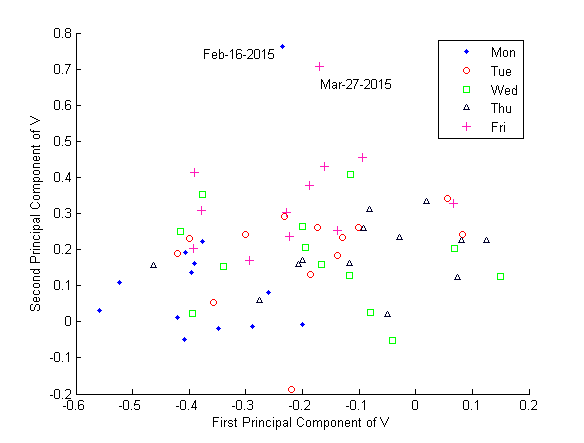
\includegraphics[scale=0.6]{VFirstTwo.png}
\caption{First and second principal component of $\mathbf{V}$}
\label{fig:VFirstTwo}
\centering
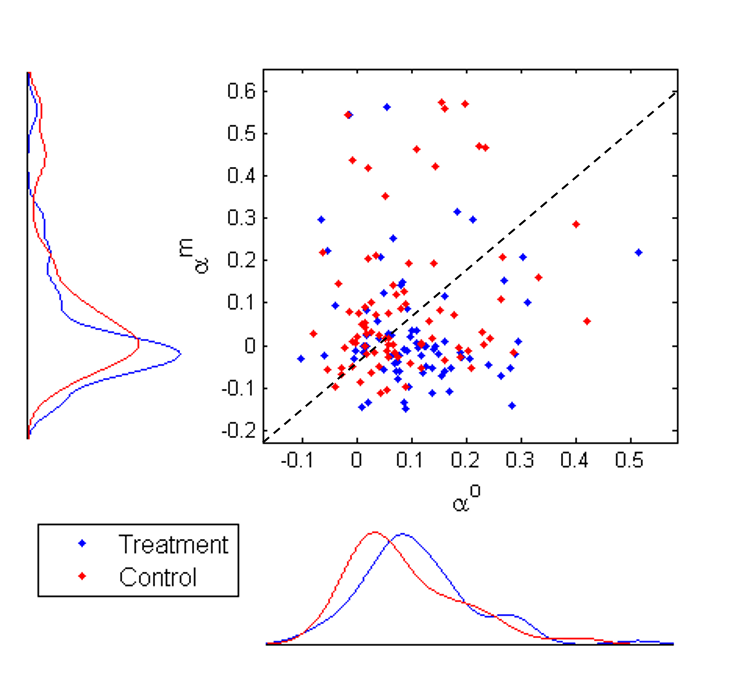
\includegraphics[scale=0.6]{ParaAlpha.png}
\caption{Scatter-hist plot for participant specific bias parameters $\alpha^o$ and $\alpha^m$}
\label{fig:AlphaMO}

\end{figure}

\subsection{Compensate Dropout Bias} (7-24)

\section{Conclusion} (7-24)

\end{document}
